\chapter{Programmazione del servizio online parte 2}\label{cap:Programmazione del servizio online parte 2}

\section{Creazione del sito internet}\label{sez:Creazione sito internet}

La realizzazione del sito internet è definibile a partire dalla creazione delle singole pagine che lo compongono.\\%si può suddividere nella creazione delle singole pagine che lo compongo.

\subsection{Creazione pagina di registrazione e di accesso}
L'intera produzione del sito internet è stata fatta cercando di dare più importanza ai lavori "più grossi", in modo che il progetto si sviluppi a partire da un nucleo principale per poi espandersi. In contrapposizione al  modo comune di  condurre questo genere di progetti, ovvero quello di partire dalle specifiche più "esterne" per  avere più velocemente una idea del progetto finito, convergendo in seguito verso il "nucleo".\\
Secondo la specifica del progetto, il sito doveva essere accessibile solo agli utenti registrati (verificando inoltre che la mail di registrazione fosse reale) garantendo la sicurezza dei dati personali, tramite l'implementazione delle principali difese contro gli attacchi e in caso di penetrazione i dati degli utenti presenti all'interno del "database" sarebbero dovuti essere cifrati per prevenirne l'uso illecito.\\
La prime pagine create sono state quelle di accesso e di registrazione, dato che queste due pagine verificavano vicendevolmente il corretto funzionamento reciproco.\\
\bigskip
Dopo aver studiato velocemente i linguaggi: "html", "php" e "javascript". Si da il via allo sviluppo, scrivendo la parte di codice in "php", utilizzando come paradigma quello ad oggetti, siccome mi è molto famigliare.\\
Come prima cosa viene creata una classe "utilities" nella quale poter ospitare i vari metodi utili nelle restanti parti future.\\
\bigskip
Si esplicita in questa sede che le varie classi che saranno presentate sono state divise ed ordinate in cartelle sulla base delle loro funzionalità.\\

\paragraph{Classe utilities}\leavevmode\\
La classe "utilities" (quindi il relativo file) è stata implementata in questo modo:\\
Si è deciso di dividere in file separati i metodi e le rispettive password di accesso ai servizi (come quelle per costruire le "query" del database) in modo da aumentare la sicurezza e l'ordine del codice.\\
Il primo metodo scritto è quello che permette di creare l'oggetto "mysqli" che serve per poter interagire con il database (da notare come nella porzione di codice inferiore non vi siano riportati direttamente i dati di accesso). Siccome quest'oggetto è per sua stessa statico, durante la sua l'implementazione è stato usato il "singleton pattern" per evitare che in memoria ci fossero degli oggetti duplicati.\\

\begin{lstlisting}[language=php]
	/*using singleton pattern*/
	public function getMysql(){
		if($this->mysqli == null){
			$this->mysqli = new mysqli(SERVER, USER, PASSWORD, DATABASE);
			
		}
		return $this->mysqli;
	}
\end{lstlisting}

\textcolor{black}{Successivamente sono stati scritti i metodi per cifrare e decifrare le stringe da salvare nella tabella utenti all'interno del database.}\\

\begin{lstlisting}[language=php]
/*Function to crypt a string*/
public function Encrypt($string){
	$encrypt_method = "AES-256-CBC";
	$key = hash( 'sha256', $secret_key );
	$iv = substr( hash( 'sha256', $secret_iv ), 0, 16 );
	$output = base64_encode( openssl_encrypt( $string, $encrypt_method, $key, 0, $iv ) );
	return $output;
}


/*Function to decrypt a string*/
public function Decrypt($string){
	$encrypt_method = "AES-256-CBC";
	$key = hash( 'sha256', $secret_key );
	$iv = substr( hash( 'sha256', $secret_iv ), 0, 16 );
	$output = openssl_decrypt( base64_decode( $string ), $encrypt_method, $key, 0, $iv );
	return $output;
}
\end{lstlisting}

\textcolor{black}{Sempre in questa classe è stato scritto il metodo che si occupa di inviare agli utenti la mail con il link di verifica della mail con cui ci si registra.\\
Per la costruzione del metodo sono stati usati i metodi messi a disposizione da "\href{https://github.com/PHPMailer/PHPMailer}{PHPMailer}"}.

\begin{lstlisting}[language=php]
public function SendEmail($address, $subject, $body, $altBody){
	
	$mail = new PHPMailer(true);
	
	try{
		//server settings
		$mail->SMTPDebug = 0; //SMPT::DEBUG_OFF;
		$mail->isSMTP();
		$mail->Host       = 'smtp.gmail.com';
		$mail->SMTPAuth   = true;
		$mail->Username   = 'quiz.patenti.nautiche@gmail.com';
		$mail->Password   = MAIL_PASSWORD;
		$mail->SMTPSecure = PHPMailer::ENCRYPTION_SMTPS;
		$mail->Port       = 465;
		
		//Recipients
		$mail->setFrom('quiz.patenti.nautiche@gmail.com', 'Quiz Patenti Nautiche');
		$mail->addAddress($address);
		
		//Content
		$mail->isHTML(true);
		$mail->Subject = $subject;
		$mail->Body = $body;
		$mail->AltBody = $altBody;
		
		//Send
		$mail->send();
		
		echo "Message has been sent";
	}catch (Exception $e){
		echo "Message could not be sent. Mailer Error: {$mail->ErrorInfo}";
	}
}
\end{lstlisting}

\textcolor{black}{
\textbf{Approfondimento gestione della verifica della mail di registrazione}\\
A questo punto si desidera aprire una breve parentesi per approfondire la gestione del processo di verifica della mail.\\
Nella classe "Utilities" è possibile trovare il metodo che permette l'invio della mail di verifica, gli argomenti in ingresso del metodo sono rispettivamente: l'indirizzo mail del destinatario ( prelevato dal database), l'oggetto della mail e i restanti argomenti si reperiscono da un'altra classe chiamata "MailUtilities".}\\

\paragraph{\textcolor{black}{classe MailUtilities}}\leavevmode\\

\textcolor{black}{Come prima cosa è stato definito un "link base di rientro" che se cliccato permette di ritornare alla pagina principale del sito.}\\

 \begin{lstlisting}[language=php]
	const URL = "https://quizpatentinautiche.dynamic-dns.net:8080/";
 \end{lstlisting}
 
  \textcolor{black}{Successivamente è stato scritto un metodo per reperire l'oggetto della mail, si è preferito scriverlo in questa classe per tenere raggruppati i vari argomenti necessari per l'invio della mail.}\\
 
\begin{lstlisting}[language=php]
public function getSubject(){
	return "Verifica della mail.";
}
\end{lstlisting}

\textcolor{black}{Di seguito è stato definito il corpo "html" della mail, il quale (per un motivo poco chiaro) non viene visualizzato correttamente su alcuni gestori online di servizi mail. }\\

\begin{lstlisting}[language=php]
public function getBody($linkToUse){
	return '<html>
	<head>
	<meta http-equiv="Content-Type" content="text/html; charset=utf-8" />
	</head>
	<body style="background-color: #e9ecef;">
	<div class="login-form" style="background: #fff;
	width: 500px; margin: 65px auto; display: -webkit-box;
	display: flex; flex-direction: column; border-radius: 4px;
	box-shadow: 0 2px 25px rgba(0, 0, 0, 0.2);">
	<form method="post">
	<h1 style="padding: 35px 35px 0 35px; font-weight: 300;
	font-family: "Rubik", sans-serif; text-align: center;">
	Verifica la tua mail
	</h1>
	<div style="margin: 25px auto; padding: 18px;
	font-family: "Rubik", sans-serif; text-align: center;">
	Clicca su questo pulsante per accedere alla pagina di verifica della mail inserita su:
	<a href='.self::URL.'>Quiz Patenti Nautiche</a>
	</div>
	<div>
	<a href='.$linkToUse.'>
	<button style="width: 250px; height: 50px; border: none;
	border-radius: 4px; padding: 18px; font-family: "Rubik", sans-serif;
	font-size: large; cursor: pointer; background: #2d3b55; color: #fff;
	letter-spacing: 0.2px; outline: 0; position: relative; top: 50\%;
	left: 50\%; -ms-transform: translate(-50\%, -50\%); transform: translate(-50\%, -50\%);">
	Verifica la tua Mail
	</button>
	</a>
	</div>
	</form>
	</div>
	</body>	</html>';
}
 \end{lstlisting}
 
 \textcolor{black}{Per ultimo si è definito un corpo alternativo nel caso in cui l'utente non voglia una visualizzazione in "html".}\\
 
  \begin{lstlisting}[language=php]
 public function getAlternativeBody($linkToUse){
 	return 'Usa questo link per accedere alla pagina di verifica della mail: '.$linkToUse;
 }
  \end{lstlisting}
  
  \textcolor{black}{Sono stati inoltre scritti dei metodi aggiuntivi per facilitare la gestione  "dell'url" usato per la verifica della mail.}\\
  
 \begin{lstlisting}[language=php]
   	public function getUrl($myData){
   		return self::URL."?".http_build_query($myData);
   	}
   	
   	public function getInfoFromUrl($url){
   		$url_component = parse_url($url);
   		parse_str($url_component['query'], $params);
   		return $params;
   	}
 \end{lstlisting}
 
 \textcolor{black}{Per spiegare più facilmente il funzionamento del processo appena presentato,  viene riportato inferiormente una parte di codice della pagina di registrazione che sfrutta i metodi presentati sopra per mandare la mail di verifica dopo la registrazione.}\\ 
 
 \begin{lstlisting}[language=php]
 $mailUtil = new MailUtilities();
 
 $tempArray = array("email" => $email);
 
 $URLToSend = $mailUtil->getURL($tempArray);
 
 $utilities->SendEmail($_POST['email'], $mailUtil->getSubject(), $mailUtil->getBody($URLToSend), $mailUtil->getAlternativeBody($URLToSend));
 /*--- Return to main page ---*/
 $_SESSION['user'] = "Registrated";
 header("Location: main.php");
 exit;
  \end{lstlisting}
  
 \textcolor{black}{ In pratica (dopo aver controllato la consistenza dei dati nel database) la mail di destinazione viene presa direttamente dal campo di testo della pagina, l'oggetto della mail da inviare è prelevato dal rispettivo metodo, mentre "l'url" che verrà usato nel corpo della mail (generato usando il metodo "getUrl") sarà l'unione del link base di accesso al sito con in aggiunta (come argomento "nell'url") la mail cifrata dell'utente stesso da usare per fare poi l'accesso al database dalla pagina di verifica della mail.\\
 In particolare (come mostrato dal codice riportato inferiormente) per favorire questo processo, la pagina posizionata a livello di "root" non è quella di accesso, ma bensì una pagina che a seconda se "nell'url" con il quale si fa l'acceso al sito è presente un argomento o meno effettua un "redirect" alla giusta pagina.}\\
  
 \paragraph{\textcolor{black}{File index.php}}\leavevmode\\
  
 \begin{lstlisting}[language=php]
 <?php
 require 'Quiz-Patente-Nautica/Pagina_Web/ValidationMail/mailUtilities.php';
 
 session_start();
 
 $urlUtility = new MailUtilities();
 $array = $urlUtility->getInfoFromUrl($_SERVER['REQUEST_URI']);
 
 if( $array['email']!== null){	
 	
 	$_SESSION['email'] = $array['email'];
 	header("location:Quiz-Patente-Nautica/Pagina_Web/ValidationMail/verificationMail.php");
 	exit;
 }else{
 	header("Location:Quiz-Patente-Nautica/Pagina_Web/main.php");
 	exit;
 }
 ?>
 \end{lstlisting}
 
 \textcolor{black}{Ecco il comportamento della pagina di verifica della mail nel caso in cui "nell'url" ci sia un argomento.}\\
 
\paragraph{\textcolor{black}{Estratto dalla pagina di verifica della mail: "verificationMail.php"}}\leavevmode\\
 
 \begin{lstlisting}[language=php]
 /*verify if mail verification has not been did yet*/
 
 $query = $utilities->getMysql()->query("SELECT verified FROM user_table1 WHERE (email = '{$_SESSION['email']}')");
 $tempArray = $query->fetch_array(MYSQLI_ASSOC);
 
 //redirect in positive case
 
 if($tempArray['verified'] == true){
 	$_SESSION['user'] = "Verified";
 	$_SESSION['email'] = null;
 	header("location:../main.php");
 	exit;
 	
 }
 
 $query = $utilities->getMysql()->query("SELECT id FROM user_table1 WHERE (email = '{$_SESSION['email']}')");
 $tempArray = $query->fetch_array(MYSQLI_ASSOC);
 
 /*verify if mail is correct*/
 if($tempArray['id'] == null){
 	$_SESSION['user'] = "NoMail";
 	header("location:../main.php");
 	exit;
 }
 
 /*confirm the mail*/
 
 if(isset($_POST['confirm'])){
 	
 	$temp = $utilities->getMysql()->query("UPDATE user_table1 SET verified = 1 WHERE (id = '{$tempArray['id']}')");
 	
 	if(!$temp){
 		$_SESSION['user'] = "DatabaseError";
 		$_SESSION['email'] = null;
 		header("location:../main.php");
 		exit;
 	}
 	
 	$query = $utilities->getMysql()->query("SELECT verified FROM user_table1 WHERE (email = '{$_SESSION['email']}')");
 	$tempArray = $query->fetch_array(MYSQLI_ASSOC);
 	
 	if($tempArray['verified'] == true){
 		$_SESSION['user'] = "YesMail";
 		$_SESSION['email'] = null;
 		header("location:../main.php");
 		exit;
 		
 	}else{
 		$_SESSION['user'] = "DatabaseError";
 		$_SESSION['email'] = null;
 		header("location:../main.php");
 		exit;
 	}
 }
 \end{lstlisting}
 
 \textcolor{black}{Il funzionamento è il seguente,  prima di tutto viene verificato che l'operazione di verifica non sia stata fatta in passato, successivamente si aspetta che l'utente prema il pulsante di verifica per aggiornare il database.}\\
 \bigskip
 \textcolor{black}{A questo punto della spiegazione è possibile introdurre il codice della pagina di registrazione (pagina raggiungibile solo attraverso quella di accesso tramite la pressione dell'apposito pulsante).\\
 Per prima cosa verrà incluso il codice in "php" in modo da poter capire il suo funzionamento e poi successivamente verrà introdotto il codice "html" per mostrare come è strutturata la pagina.}\\
 
 %% Insert verification mail page here %%
 
 \paragraph{\textcolor{black}{registration.php}}\leavevmode\\
 
 \begin{lstlisting}[language=php]
 <?php
 //require 'Utilities/keys.php';
 require 'Utilities/utilities.php';
 require 'ValidationMail/mailUtilities.php';
 
 /*get utility available*/
 $utilities = new Utilities();
 
 /*Starting session*/
 session_start();
 
 /*check if  database is reachable*/
 if ($utilities->getMysql()->connect_errno) {
 	die('Impossible conncet to database'.$utilities->getMysql()->connect_error);
 }
 
 if(isset($_POST['register'])){
 	
 	if(filter_has_var(INPUT_POST, 'agree')){
 		
 		if(!empty($_POST['name']) && !empty($_POST['surname']) && !empty($_POST['email']) && !empty($_POST['password1']) && !empty($_POST['password2'])){
 			
 			if($_POST['password1'] == $_POST['password2']){
 				
 				/*extract all fields to use*/
 				$name = $utilities->Encrypt($_POST['name']);
 				$surname = $utilities->Encrypt($_POST['surname']);
 				$email = $utilities->Encrypt($_POST['email']);
 				$password = $utilities->Encrypt($_POST['password1']);
 				
 				/*make query to register new dates*/
 				$query = $utilities->getMysql()->query("INSERT INTO user_table1 (name, surname, email, password) VALUES ('{$name}', '{$surname}', '{$email}', '{$password}')");
 				
 				/*verify if query worked*/
 				if(!$query){
 					die('Query failed'.$utilities->getMysql()->error);
 				}
 				
 				/*test if registration had success */
 				$query = $utilities->getMysql()->query("SELECT password FROM user_table1 WHERE (email = '{$email}')");
 				$TestPassword = $query->fetch_array(MYSQLI_ASSOC)['password'];
 				
 				/*verify if passwords are equal*/
 				if($password === $TestPassword){
 					
 					/*--- Send evrification mail ---*/
 					
 					$mailUtil = new MailUtilities();
 					
 					$tempArray = array("email" => $email);
 					
 					$URLToSend = $mailUtil->getURL($tempArray);
 					
 					$utilities->SendEmail($_POST['email'], $mailUtil->getSubject(), $mailUtil->getBody($URLToSend), $mailUtil->getAlternativeBody($URLToSend));
 					/*--- Return to the main page ---*/
 					$_SESSION['user'] = "Registered";
 					header("Location: main.php");
 					exit;
 					
 				}else{
 					$query = $utilities->getMysql()->query("DELETE * FROM usert_table1 WHERE (email = '{$email}')");
 					
 					if(!$query){
 						die('Query failed'.$utilities->getMysql()->error);
 					} 
					$utilities->Popup("La registrazione ha dato esito negativo");
 				}
 			}else{
 				$utilities->Popup("Le password non corrispondono");
 			}
 		}else{
 			$utilities->Popup("I campi devono essere tutti riempiti");
 		}
 	}else{
 		$utilities->Popup("Devi accettare i termini di utilizzo");
 	}
 }
 
 /*Return to main page page*/
 if(isset($_POST['cancel'])){
 	header("Location: main.php");
 	exit;
 }
 
 ?>
 \end{lstlisting}
 
 \textcolor{black}{Osservando le classi incluse si può notare che è presente quella che gestisce l'invio della mail, in modo da poter (subito dopo aver completato la prima fase di registrazione) inviare una mail per la verifica dell'utente.\\
 Si avvia la sessione per non perdere lo stato della memoria (di conseguenza quello dell'utente) nello spostamento tra le varie pagine.\\
 Siccome questa pagina fa uso del database, si controlla che la connessione a quest'ultimo.\\
 A questo punto compare una serie di "if" annidati che anche se rendono la lettura del codice più difficile, offrono una maggiore garanzia che la pagina non abbia dei comportamenti anomali, cosa che potrebbe accadere nel momento in cui ogni "if" fosse posto in sequenza.\\
 Come ultima cosa a fine registrazione s'imposta nella sessione lo stato "registered" in modo da poter poi far apparire nella pagina principale il messaggio di registrazione avvenuta.}\\
 
 \begin{lstlisting}[language=html]
 	<!DOCTYPE html>
 	<html lang="it" >
 	<head>
 	<meta charset="UTF-8">
 	<title>Registrazione</title>
 	<link rel='stylesheet' href='https://fonts.googleapis.com/css?family=Rubik:400,700'><link rel="stylesheet" href="style.css">
 	
 	</head>
 	<body>
 	<!-- Welocome text -->
 	<div class="welcomeText">
 	<h1>Quiz patenti nautiche DD 131 del 31 Maggio 2022</h1>
 	</div>
 	<!-- Login form -->
 	<div class="login-form">
 	<form method="post">
 	<h1>Inserisci i dati richiesti</h1>
 	<div class="content">
 	<div class="input-field">
 	<input type="text" name="name" placeholder="Nome">
 	</div>
 	<div class="input-field">
 	<input type="text" name="surname" placeholder="Cognome">
 	</div>
 	<div class="input-field">
 	<input type="email" name="email" placeholder="Email">
 	</div>
 	<div class="input-field">
 	<input type="password" name="password1" placeholder="Password">
 	</div>
 	<div class="input-field">
 	<input type="password" name="password2" placeholder="Ripeti Password">
 	</div>
 	</div>
 	<div class="checkbox">
 	<input type="checkbox" name="agree" value ="agree"/>
 	<label for="agree"> Accetto i <a href="Terms&Services/terms&Services.html">Termini</a> di utilizzo</label>
 	</div>
 	<div class="action">
 	<input type="submit" name="register" value="Registrati" id="button2"/>
 	<input type="submit" name="cancel" value="Annulla" id="button1"/>
 	</div>
 	</form>
 	</div>
 	
 	</body>
 	</html>
  \end{lstlisting}
  
  \textcolor{black}{Nella parte in "html" della pagina si possono notare i vari oggetti che sono stati istanziati per essere poi interagiti tramite la parte in "php".\\
  	 Da questo momento in poi, raramente verrà incluso il codice "html" delle pagine siccome quest'ultimo non varia molto. Verranno invece evidenziate soltanto le parti degne di nota.}\\
  
 \begin{figure}[h]
 	\begin{center}
 		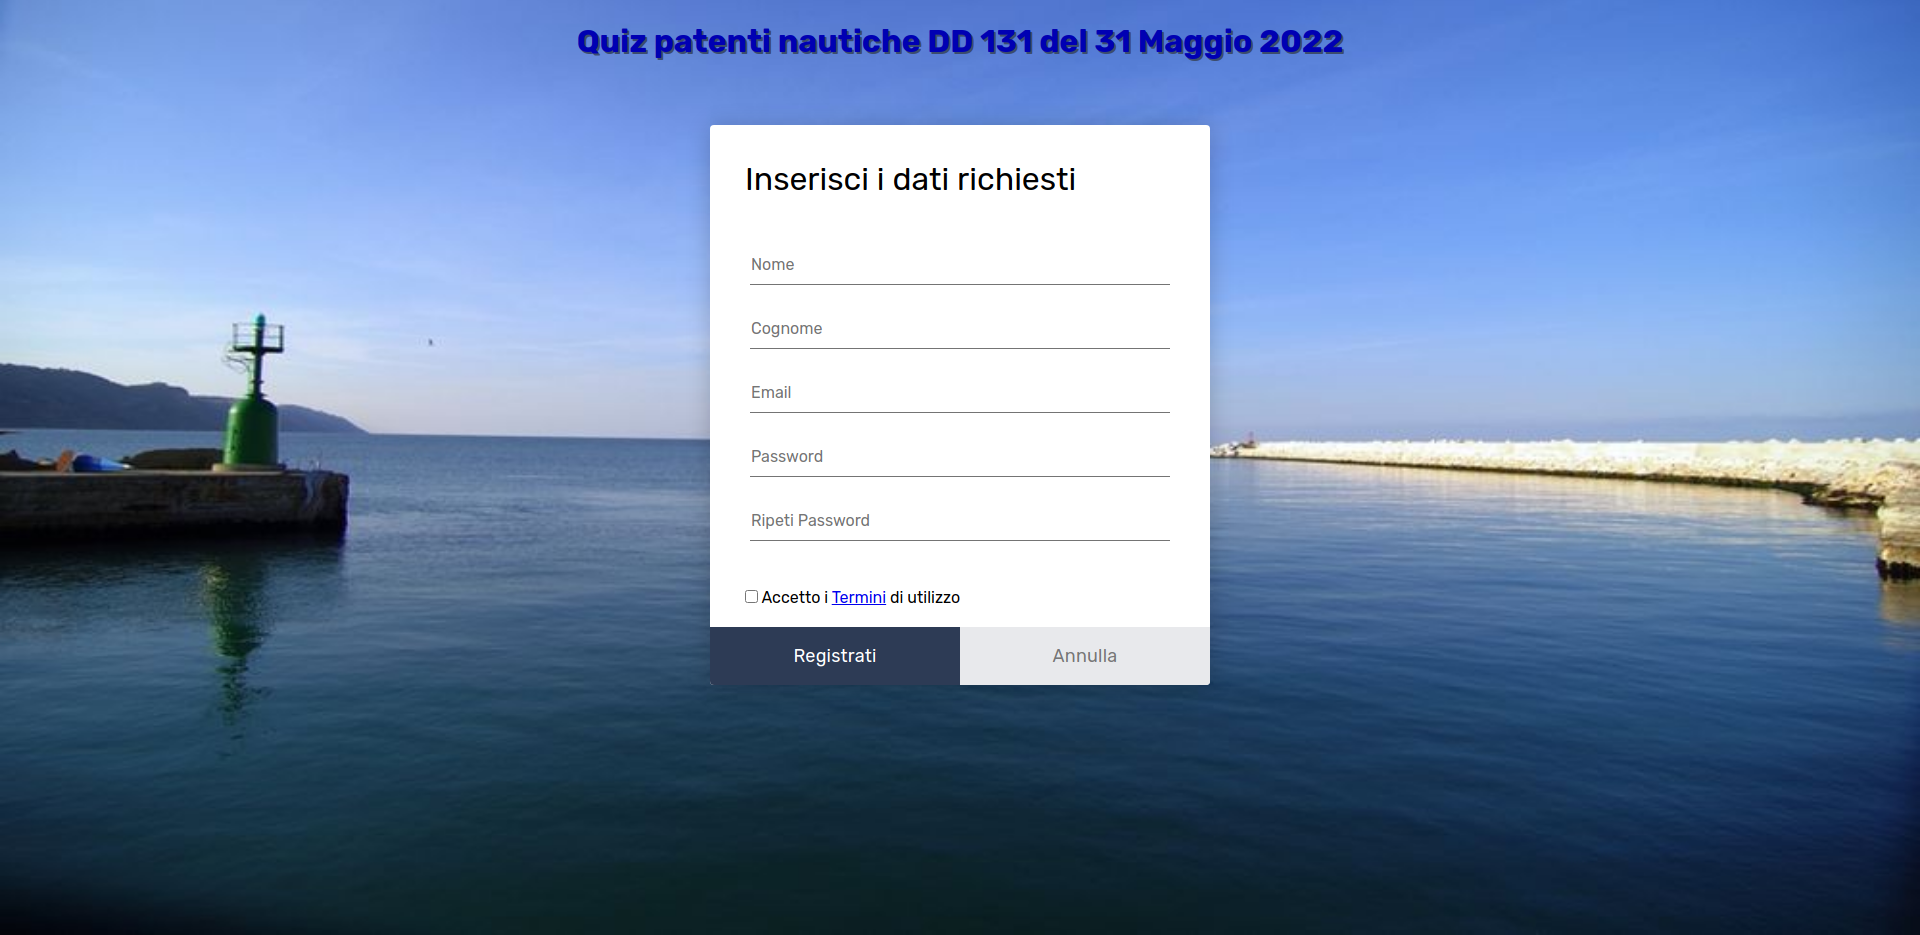
\includegraphics[scale=0.25]{Sites-images/03-Pagina_di_registrazione.png}
 		\caption{Pagina di registrazione.}
 	\end{center}
 \end{figure}
  
  \textcolor{black}{Vista ora la pagina di registrazione, si può procedere con l'analisi della pagina di accesso.}\\
  
  \paragraph{\textcolor{black}{main.php}}\leavevmode\\
  
  \textcolor{black}{Nel codice di questa pagina si può notare che durante l'intero sviluppo della applicazione web è stata prestata particolare attenzione alla scrittura di un codice efficiente in modo non solo di poter risparmiare risorse sul "RaspberryPi" ma anche con l'intento di rendere la navigazione più "responsive". Si è cercato di ridurre al minimo le interazioni tra "server" e "client" con l'intento di alleggerire il costo delle varie connessioni in modo da garantire a più utenti una esperienza di navigazione soddisfacente. Nel caso specifico di questa pagina (il cui codice è riportato) la gestione dei veri avvisi è stata fatta utilizzando lo "switch" rispetto ad una serie di "if" in cascata, tenendo presente che il comportamento del sito non sarebbe cambiato a prescindere dall'uso di uno dei due sistemi. ma in questo modo si è visto (utilizzando l'applicazione "\href{https://htop.dev/}{HTOP}") che l'accesso al sito pesava meno sul "core" della macchina che è stato scelto dal sistema operativo per elaborare la richiesta.}\\
  
 \begin{lstlisting}[language=php]
 /*reset latest connection*/
 $_SESSION['mail'] = null;
 $_SESSION['password'] = null;
 
 /*check if database connection is okay*/
 if ($utilities->getMysql()->connect_errno) {
 	die('Unable to connect to database'. $utilities->getMysql()->connect_error);
 }
 
 /*Verify status*/
 switch($_SESSION['user']){
 	case "Registered":
 	$utilities->Popup("La registrazione e' avvenuta con successo");
 	$utilities->Popup("La mail per verificare l`account e stata inviata");
 	$_SESSION['user'] = null;
 	break;
 	
 	case "MailSend":
 	$utilities->Popup("La mail per verificare l`account e' stata inviata");
 	$_SESSION['user'] = null;
 	break;
 	
 	case "NoMail":
 	$utilities->Popup("Non e' stato possibile confermare la mail");
 	$_SESSION['user'] = null;
 	break;
 	
 	case "YesMail":
 	$utilities->Popup("La mail e' stata confermata con successo");
 	$_SESSION['user'] = null;
 	break;
 	
 	case "DatabaseError":
 	$utilities->Popup("Errore durante l`aggiornamento del database");
 	$_SESSION['user'] = null;
 	break;
 	
 	case "Verified":
 	$utilities->Popup("La mail e' gia' stata verificata");
 	$_SESSION['user'] = null;
 	break;
 	
 	case "YesDelete":
 	$utilities->Popup("L`account e' stato eliminato con successo");
 	$_SESSION['user'] = null;
 	break;
 	
 	case "NoDelete":
 	$utilities->Popup("Non e' stato possibile eliminare l`account");
 	$_SESSION['user'] = null;
 	break;
 	
 	case "NotAllow":
 	$utilities->Popup("Non si possiedono i permessi per poter accedere alla pagina");
 	$_SESSION['user'] = null;
 	break;
 }
\end{lstlisting}

 \textcolor{black}{Viene ora riportata senza commenti (poiché superflui data la natura del codice) la porzione che si occupa di gestire l'autenticazione dell'utente.}\\ 

\begin{lstlisting}[language=php]
	/*when login button is clicked*/
	if(isset($_POST['enter'])){
		
		if(!empty($_POST['email']) && !empty($_POST['password'])){
			
			$email = $utilities->Encrypt($_POST['email']);
			$query = $utilities->getMysql()->query("SELECT password, verified FROM user_table1 WHERE (email = '{$email}')");
			
			/*check query correctness*/
			if(!$query){
				$utilities->Popup("Errore durante l'accesso alle informazioni");
				exit;
			}
			
			/*extract my aray*/
			$tempArray = $query->fetch_array(MYSQLI_ASSOC);
			
			$verified = $tempArray['verified'];
			/*extract the password from query*/
			$password = $tempArray['password'];
			
			/*verify account esistence*/  
			if($password !== null){
				
				/*check mail verification*/
				if($verified !== null && $verified == true){
					
					/*verify password correctness*/
					if($utilities->Decrypt($password) === $_POST['password']){
						$_SESSION['mail'] = $email;
						$_SESSION['password'] = $password;
						header("Location: Course/entry.php");
						exit;
						
					}else{
						$utilities->Popup("Le credenziali inserite non sono corrette");
					}
					
				}else{
					$utilities->Popup("La mail dell`account non e stata verificata.");
				}
				
			}else{
				$utilities->Popup("L`account non esite");
			}
			
		}else{
			$utilities->Popup("I campi devono essere tutti riempiti");
		}
	}
\end{lstlisting}

\begin{figure}[h]
	\begin{center}
		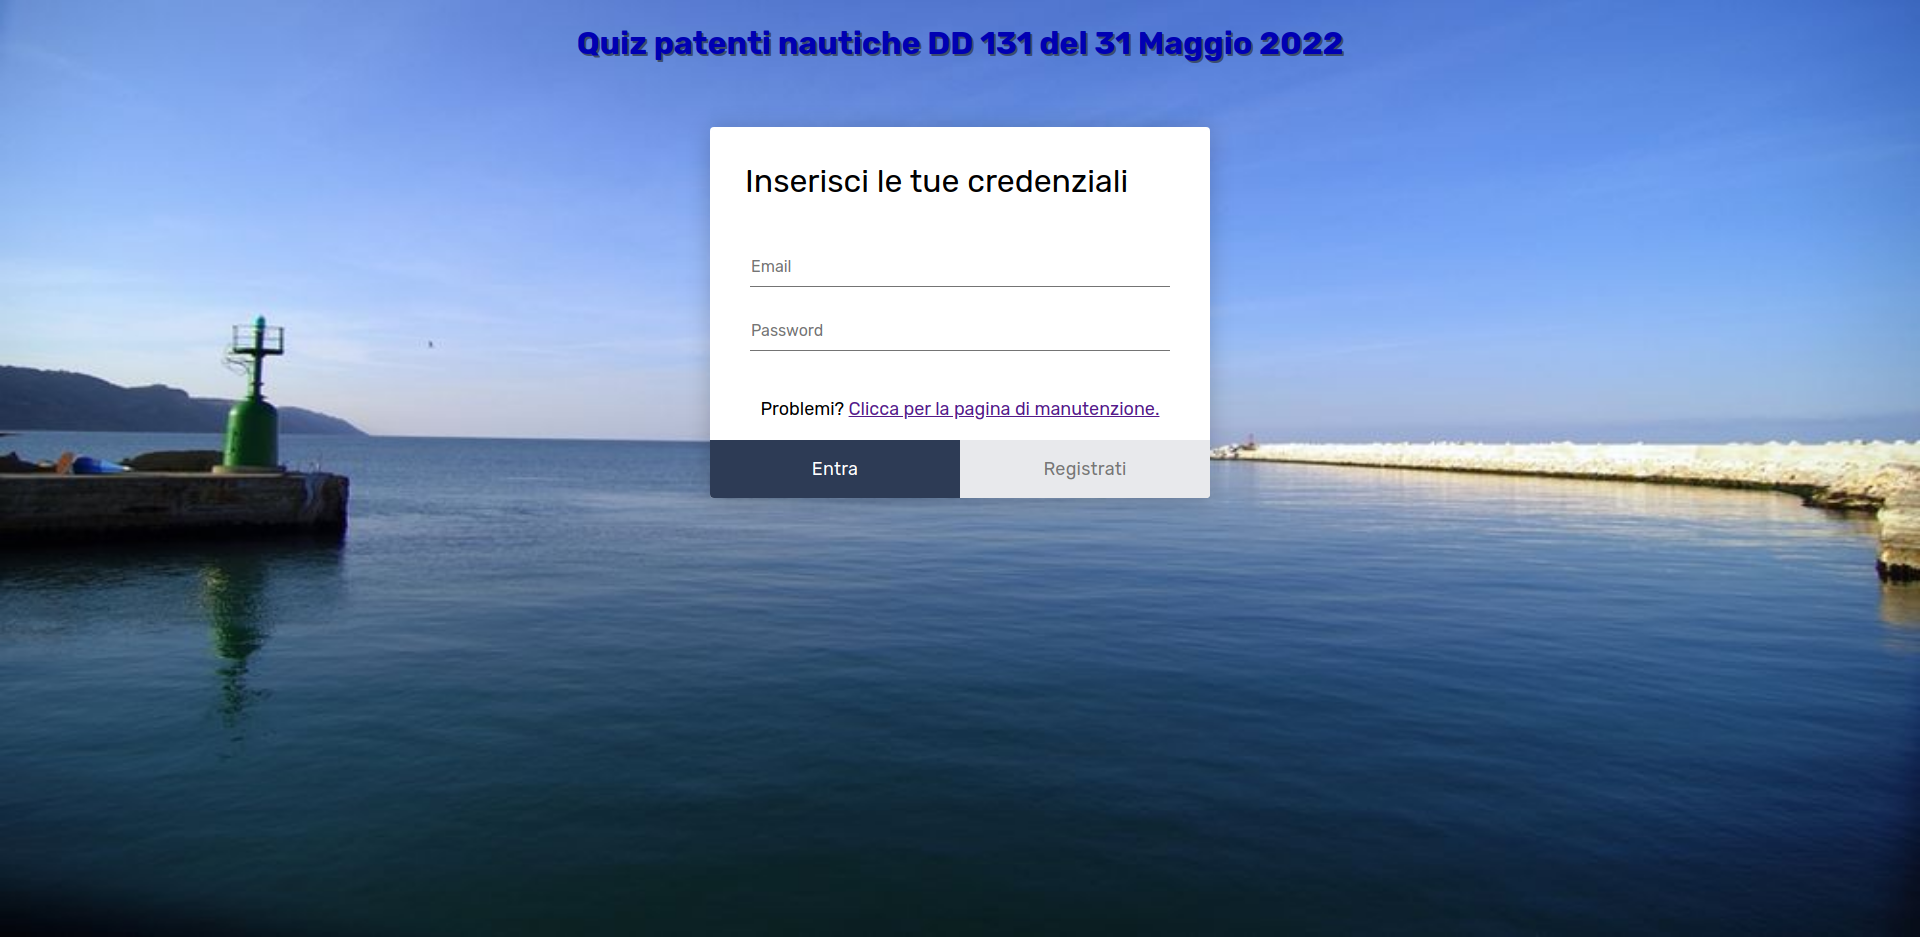
\includegraphics[scale=0.25]{Sites-images/01-Home_sito.png}
		\caption{Pagina d'accesso.}
	\end{center}
\end{figure}

\subsection{Pagina di manutenzione}
\textcolor{black}{Finora è stata mostrata la registrazione e l'autenticazione dell'utente, ma nel sito è anche disponibile una pagina (della quale si riporta inferiormente il codice in "php") che permette la manutenzione dell'account ("on-fly").}\\

\paragraph{\textcolor{black}{maintenance.php}}\leavevmode\\

\begin{lstlisting}[language=php]
	/*function to verify if credentials are okay*/
	function verifyAccount(){
		
		if(!empty($_POST['email']) && !empty($_POST['password'])){
			
			$email = $GLOBALS['utilities']->Encrypt($_POST['email']);
			$query = $GLOBALS['utilities']->getMysql()->query("SELECT password FROM user_table1 WHERE (email = '{$email}')");
			
			/*verify query correctness*/
			if(!$query){
				$GLOBALS['utilities']->Popup("Errore nel accedere alle informazioni");
				exit;
			}
			
			/*extract password*/
			$password = $query->fetch_array(MYSQLI_ASSOC)['password'];
			
			/*verify account existence*/
			if($password !== null){
				
				if($GLOBALS['utilities']->Decrypt($password) === $_POST['password']){
					
					return true;
					
				}else{
					$GLOBALS['utilities']->Popup("Le credenziali inserite non sono corrette");
					return false;
				}
				
			}else{
				$GLOBALS['utilities']->Popup("L`account non esite");
				return false;
			}
			
		}else{
			$GLOBALS['utilities']->Popup("Per procedere con l`operazione i campi devono essere tutti riempiti");
			return false;
		}
		
	}
	
	/*set status in case of account deleting*/
	if(isset($_POST['delete'])){
		
		if(verifyAccount()){
			
			/*at this point is safe remove account*/
			$email = $utilities->Encrypt($_POST['email']);
			$query = $utilities->getMysql()->query("DELETE FROM user_table1 WHERE (email = '{$email}')");
			
			if(!$query){
				$utilities->Popup("Errore durante l`eliminazione dell`account");
				exit;
			}
			
			$query = $utilities->getMysql()->query("SELECT password FROM user_table1 WHERE (email = '{$email}')");
			$password = $query->fetch_array(MYSQLI_ASSOC)['password'];
			if($password == null){
				$_SESSION['user'] = "YesDelete";
				header("Location: ../main.php");
				exit;
			}else{
				$_SESSION['user'] = "NoDelete";
				header("Location: ../main.php");
				exit;
			}
		}
		
	}
	/*In case to resend the verification email*/
	if(isset($_POST['resend'])){
		
		/*verify account*/
		if(verifyAccount()){
			$email = $utilities->Encrypt($_POST['email']);
			
			$tempArray = array("email" => $email);
			
			$URLToSend = $mailUtil->getURL($tempArray);
			
			$utilities->SendEmail($_POST['email'], $mailUtil->getSubject(), $mailUtil->getBody($URLToSend), $mailUtil->getAlternativeBody($URLToSend));
			
			$_SESSION['user'] = "MailSend";
			header("Location: ../main.php");
			exit;
			
		}
	}
\end{lstlisting}

\textcolor{black}{Una peculiarità di questa pagina è il fatto che (come premesso) le operazioni vengano fatte "on-fly". La motivazione dietro questa scelta risiede nella gestione semplificata delle operazioni più critiche, dato che è possibile riciclare del codice dalle pagine precedenti e che in questo modo si garantisce una maggiore sicurezza, siccome non è presente una sessione utente "critica" nella quale sarebbero possibili dei tentativi "Hijacking". \\
La non presenza di una sessione con tanto di pagina di "atterraggio" dove effettuare le operazioni di gestione dell'account previene questo tipo di attacchi.\\
Come si può leggere da codice, questa pagina mette a disposizione due principali operazioni: quella di farsi mandare nuovamente la mail per la verifica dell'utente e la possibilità di poter cancellare l'account.\\
A questo punto si desidera presentare come la scelta progettuale fatta risulti particolarmente efficace. Supponendo che un utente volesse fare il rinvio della mail di verifica, questa operazione implicherebbe che la mail dell'utente debba rimanere in sessione (dopo aver effettuato l'acceso) in modo che la pagina di manutenzione possa completare l'operazione con la conseguenza di dover tenere in sessione una informazione sensibile. Per questo motivo le operazioni "on-fly" (quindi con ri-autenticazione) offrono un margine di sicurezza maggiore.}\\

\begin{figure}[h]
	\begin{center}
		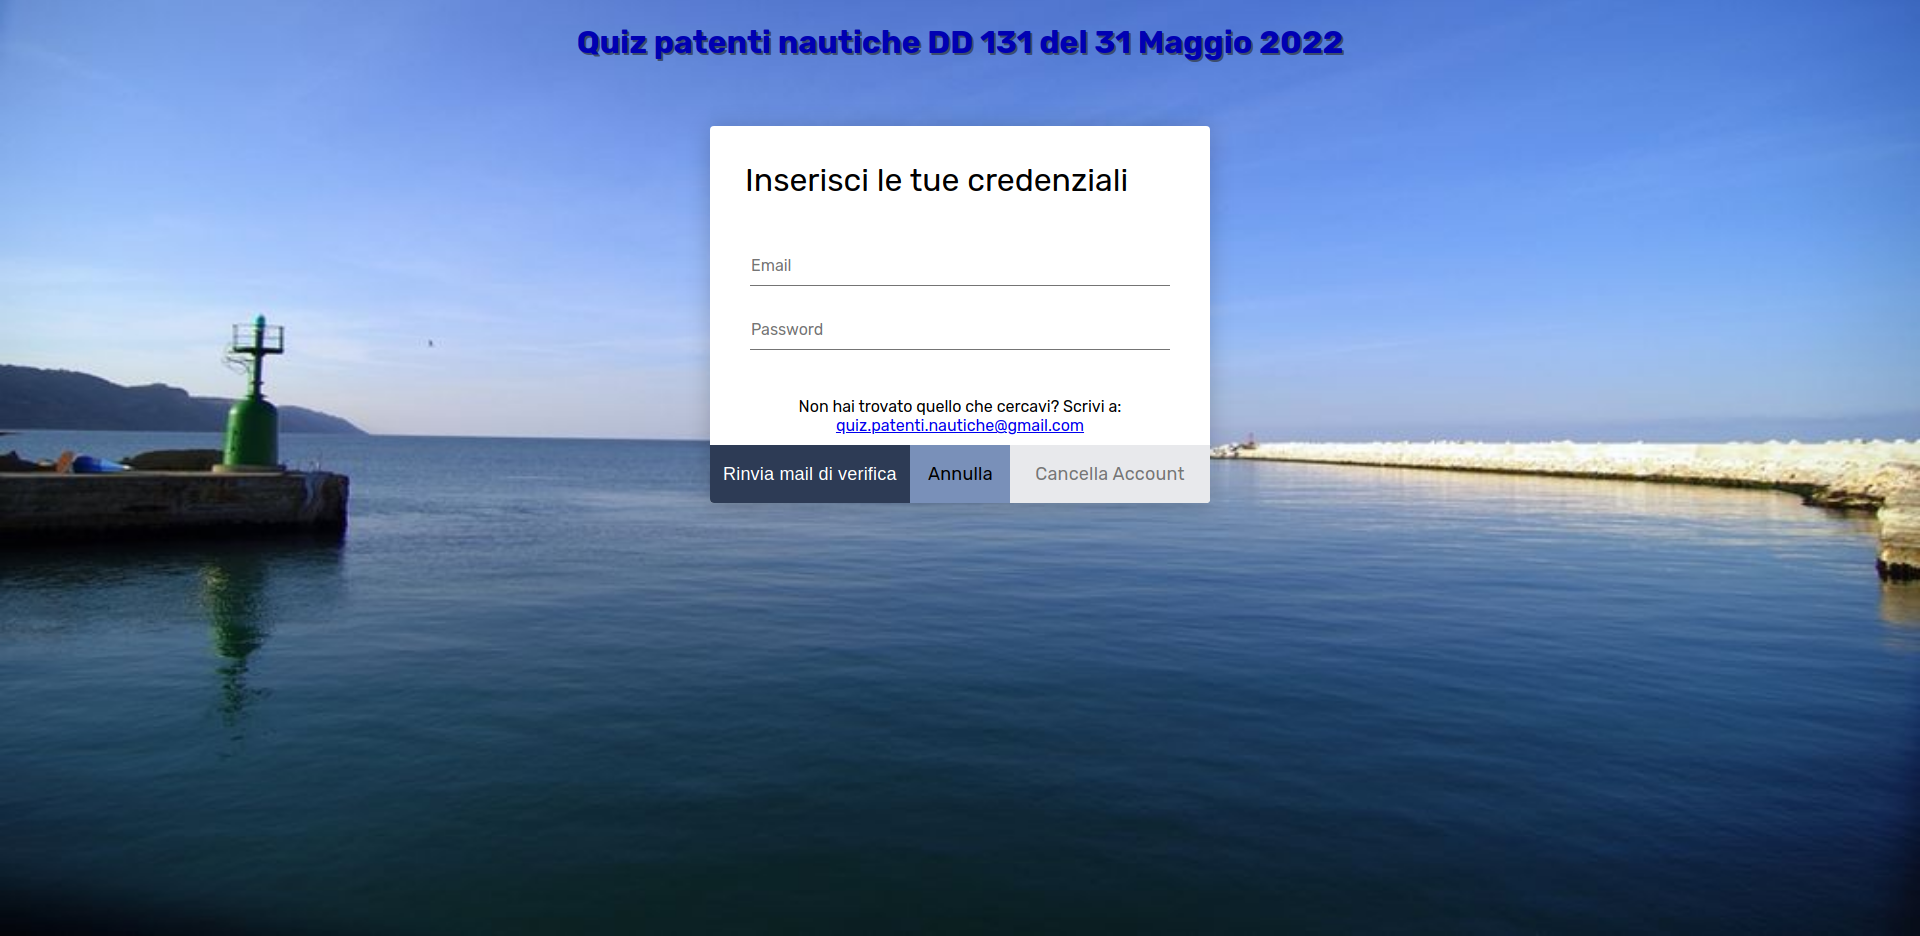
\includegraphics[scale=0.25]{Sites-images/02-Pagina_di_manutenzione.png}
		\caption{Pagina di manutenzione.}
	\end{center}
\end{figure}